\documentclass[11pt, letterpaper, article, oneside]{inrs-report} % Use this line for English report
%\documentclass[11pt, letterpaper, article, oneside, francais]{inrs-report} % Use this line for French report
\usepackage{listings}
%%% Packages %%%
\usepackage[utf8]{inputenc} % Change utf8 to latin1 on Windows, etc.
\usepackage{fourier} % Optional package to use Utopia fonts
%\usepackage[charter]{mathdesign}      % Optional package to use Bitstream Charter font.
\usepackage{csquotes}                 % Guillemets en français (context sensitive )
\usepackage{listings} % For code snippets
\usepackage{caption}
%\usepackage{minted} % For more beautiful code snippets
\usepackage{graphicx} % For imported graphs, diagrams, pictures.
\usepackage{subcaption} % For captions with multiple images
\usepackage{amsmath}
\usepackage{amssymb}
\usepackage{amsfonts}
\usepackage{float} % To put captions where I want
\usepackage[dvipsnames]{xcolor} % for the dirtree
\usepackage{dirtree} % the dirtree itself
\usepackage{mdframed} % for line breaking in code
\usepackage{subcaption}
\usepackage{forest}
\usepackage{dirtree}
\usepackage{cite}
\usepackage[framed,numbered,autolinebreaks,useliterate]{mcode}

\setlength{\parindent}{0pt}
\newcommand\myfolder[1]{{\color{#1}\rule{2ex}{2ex}}} % icons for dirtree
\renewcommand{\Re}[1]{\ensuremath{\text{Re}\left\{#1\right\}}}
\renewcommand{\Im}[1]{\ensuremath{\text{Im}\left\{#1\right\}}}
\graphicspath{ {images/} } % For emplacement of pictures.
\bibliographystyle{unsrt}
\mdfsetup{
 linecolor=black,
 topline=true,
 bottomline=true,
 leftline=false,
 rightline=false,
 backgroundcolor=yellow!20!white,
 splittopskip=2\topsep}
 \lstset{
 frameround=fttt,
 language=Bash,
 numbers=left,
 breaklines=true,
 keywordstyle=\color{darkgray}\bfseries, 
 basicstyle=\ttfamily\color{darkgray},
 numberstyle=\color{black}}
\lstMakeShortInline[columns=fixed]|



\setcounter{secnumdepth}{4}

% \titleformat{\paragraph}
% {\normalfont\normalsize\bfseries}{\theparagraph}{1em}{}
% \titlespacing*{\paragraph}
% {0pt}{3.25ex plus 1ex minus .2ex}{1.5ex plus .2ex}

\begin{document}

\title{Internship Report : 3D computed tomography with betatron X-ray}
% \reportnumber{1} % Space project report number
% \reportversion{3} % Optional revision number
\author{Olivier Saint-Vincent}
\supervisor{Simon Valli\`{e}res \\ Sylvain Fourmaux}
\affiliation{INRS -- Centre \'Energie-Mat\'eriaux-T\'el\'ecommunications \\ Varennes, Qu\'ebec, Canada} % rajouter poly
\logo{\includegraphics[width=0.4\textwidth]{INRS-logo}}
\date{August 1, 2025} % Date of first revision
\revision{\today} % Current revision
\setcounter{tocdepth}{4} %<--------
\setcounter{secnumdepth}{4} 
\printtitle
\newpage
\tableofcontents

\newpage

\OnehalfSpacing

\newpage
\section{Introduction}

The INRS Advanced Laser Light Source Laboratory 750TW laser has many scientific uses. Among these various utilities are plasma acceleration and, therefore, x-ray generation via laser Wakefield acceleration. By accelerating electrons through a plasma generated by the laser and then slowing them down, x-rays are created through bremsstrahlung, energy released through radiation when electrons slow down. With these x-rays, using x-ray detectors, detailed scans and tomographies can be created.
\newline

Tomography or more commonly known as computed Tomography (CT) was initially mathematically introduced in the early 20th by Johann Radon through the Radon transform and is one of the most worked on inverse problems. By taking multiple x-ray scans of an object at different angles, it is possible to reconstruct the interior of the object. The most common use of computed tomography is in the medical field in PET, MRI and CT scans.  \newline

Unlike medical technology, the geometry the inversion must consider can change. This can lead to unusual situations where analytical inversion solutions no longer work. Non-analytical iterative solutions were developed in the 70s and are still used today. With significantly faster computation speeds due to the invention of the GPU which relies on parallelization and hardware dedicated to linear algebra, reconstructions are much faster. With these faster compute speed, secondary optimization can be performed with modern machine learning to perfect the geometry's parameters.


\clearpage


\section{Methodology}

\subsection{Image pre-processing}

The initial tomographic scans obtained from detectors cannot be used to perform any reconstruction. Many corrections must be performed before the projections can be used. As previously mentioned, to ensure optimal output and consistent X-ray flux, multiple shots per angle must be taken. Two other captures must be taken for the corrections to be done properly: a gain map and an offset map. There are four main pre-processing techniques applied. The first three are applied to to each frame of each angle whilst the last is used to combine all of them.

\begin{figure}[h]
\centering
    \includegraphics[width=0.5\linewidth]{base_image.pdf}
\caption{Example of a raw scan}
\end{figure}


\begin{figure}[h]
\centering
  \begin{subfigure}{.5\textwidth}
    \includegraphics[width=1\linewidth]{gain_map.pdf}
    \caption{Gain map}
  \end{subfigure}%
    \begin{subfigure}{.5\textwidth}

    \includegraphics[width=1\linewidth]{offset_map.pdf}
    \caption{Offset map}
  \end{subfigure}%

    \caption{Example of calibration frames}
    \label{fig:calibration frames}
\end{figure}

\subsubsection{Flat-field correction}

The variation between the pixel values of each scan is very minimal; this leads to a purely gray image. A primitive way to make the image viewable would be to clip the extreme values and adjust the constrast, but this leads to a loss of fidelity and detail. Instead, a very common digital image correction technique must be applied: a flat-field correction:

\[  C = \hat{G}\cdot\frac{R - O}{G} \] 

where C is the corrected image, R is the raw image, O is the offset map, G is the gain map and \(\hat{G}\) is the average pixel value of the gain map. Each image and map can be viewed as a matrix and the division is the inverse Hadamard product.

\begin{figure}[h]
\centering
  \begin{subfigure}{.5\textwidth}
    \includegraphics[width=1\linewidth]{base_image_clipped.pdf}
    \caption{Contrast adjusted}
  \end{subfigure}%
  \begin{subfigure}{.5\textwidth}
    \includegraphics[width=1\linewidth]{gain_corrected.pdf}
    \caption{Flat-field corrected}
  \end{subfigure}%
\caption{Comparison of contrast adjusted and flat-field corrected images}
\label{fig:Comparison}
\end{figure}



\subsubsection{Bad pixel correction}

Bad pixels are pixels that are considered defective. To be considered defective, the detectors' sensors can have faulty values or be completely non-functional. To determine which pixels are bad, the following algorithm is applied. \newline

Initially, two values must be set: kernel size and the comparison ratio. The algorithm starts by obtaining the average map from the gain map. The average map is obtained by taking the average of the nearest neighbors based on the kernel size previously set. Once the average map is obtained, each pixel in the gain map is compared to its respective pixel in the average map. Should the ratio between these two be larger than our comparison ratio, the pixel is considered a bad pixel (figure \ref{fig:Bad pixel pipeline}).\newline

Once the bad pixels are found, another nearest neighbor approach is taken. In our flat-field corrected frames, for each bad pixel, if in the 8 adjacent pixels there exists a good pixel, then our bad pixel will be replaced by the average of the good neighboring pixels (figure \ref{fig:Bad pixel correction}).

\begin{figure}[h]
   \centering      
    \includegraphics[width=0.85\textwidth, angle=0]{pipeline_bad_pixel.pdf}
 \caption{Bad pixel map generation pipeline}
 \label{fig:Bad pixel pipeline}
\end{figure}

\begin{figure}[h]
   \centering      
    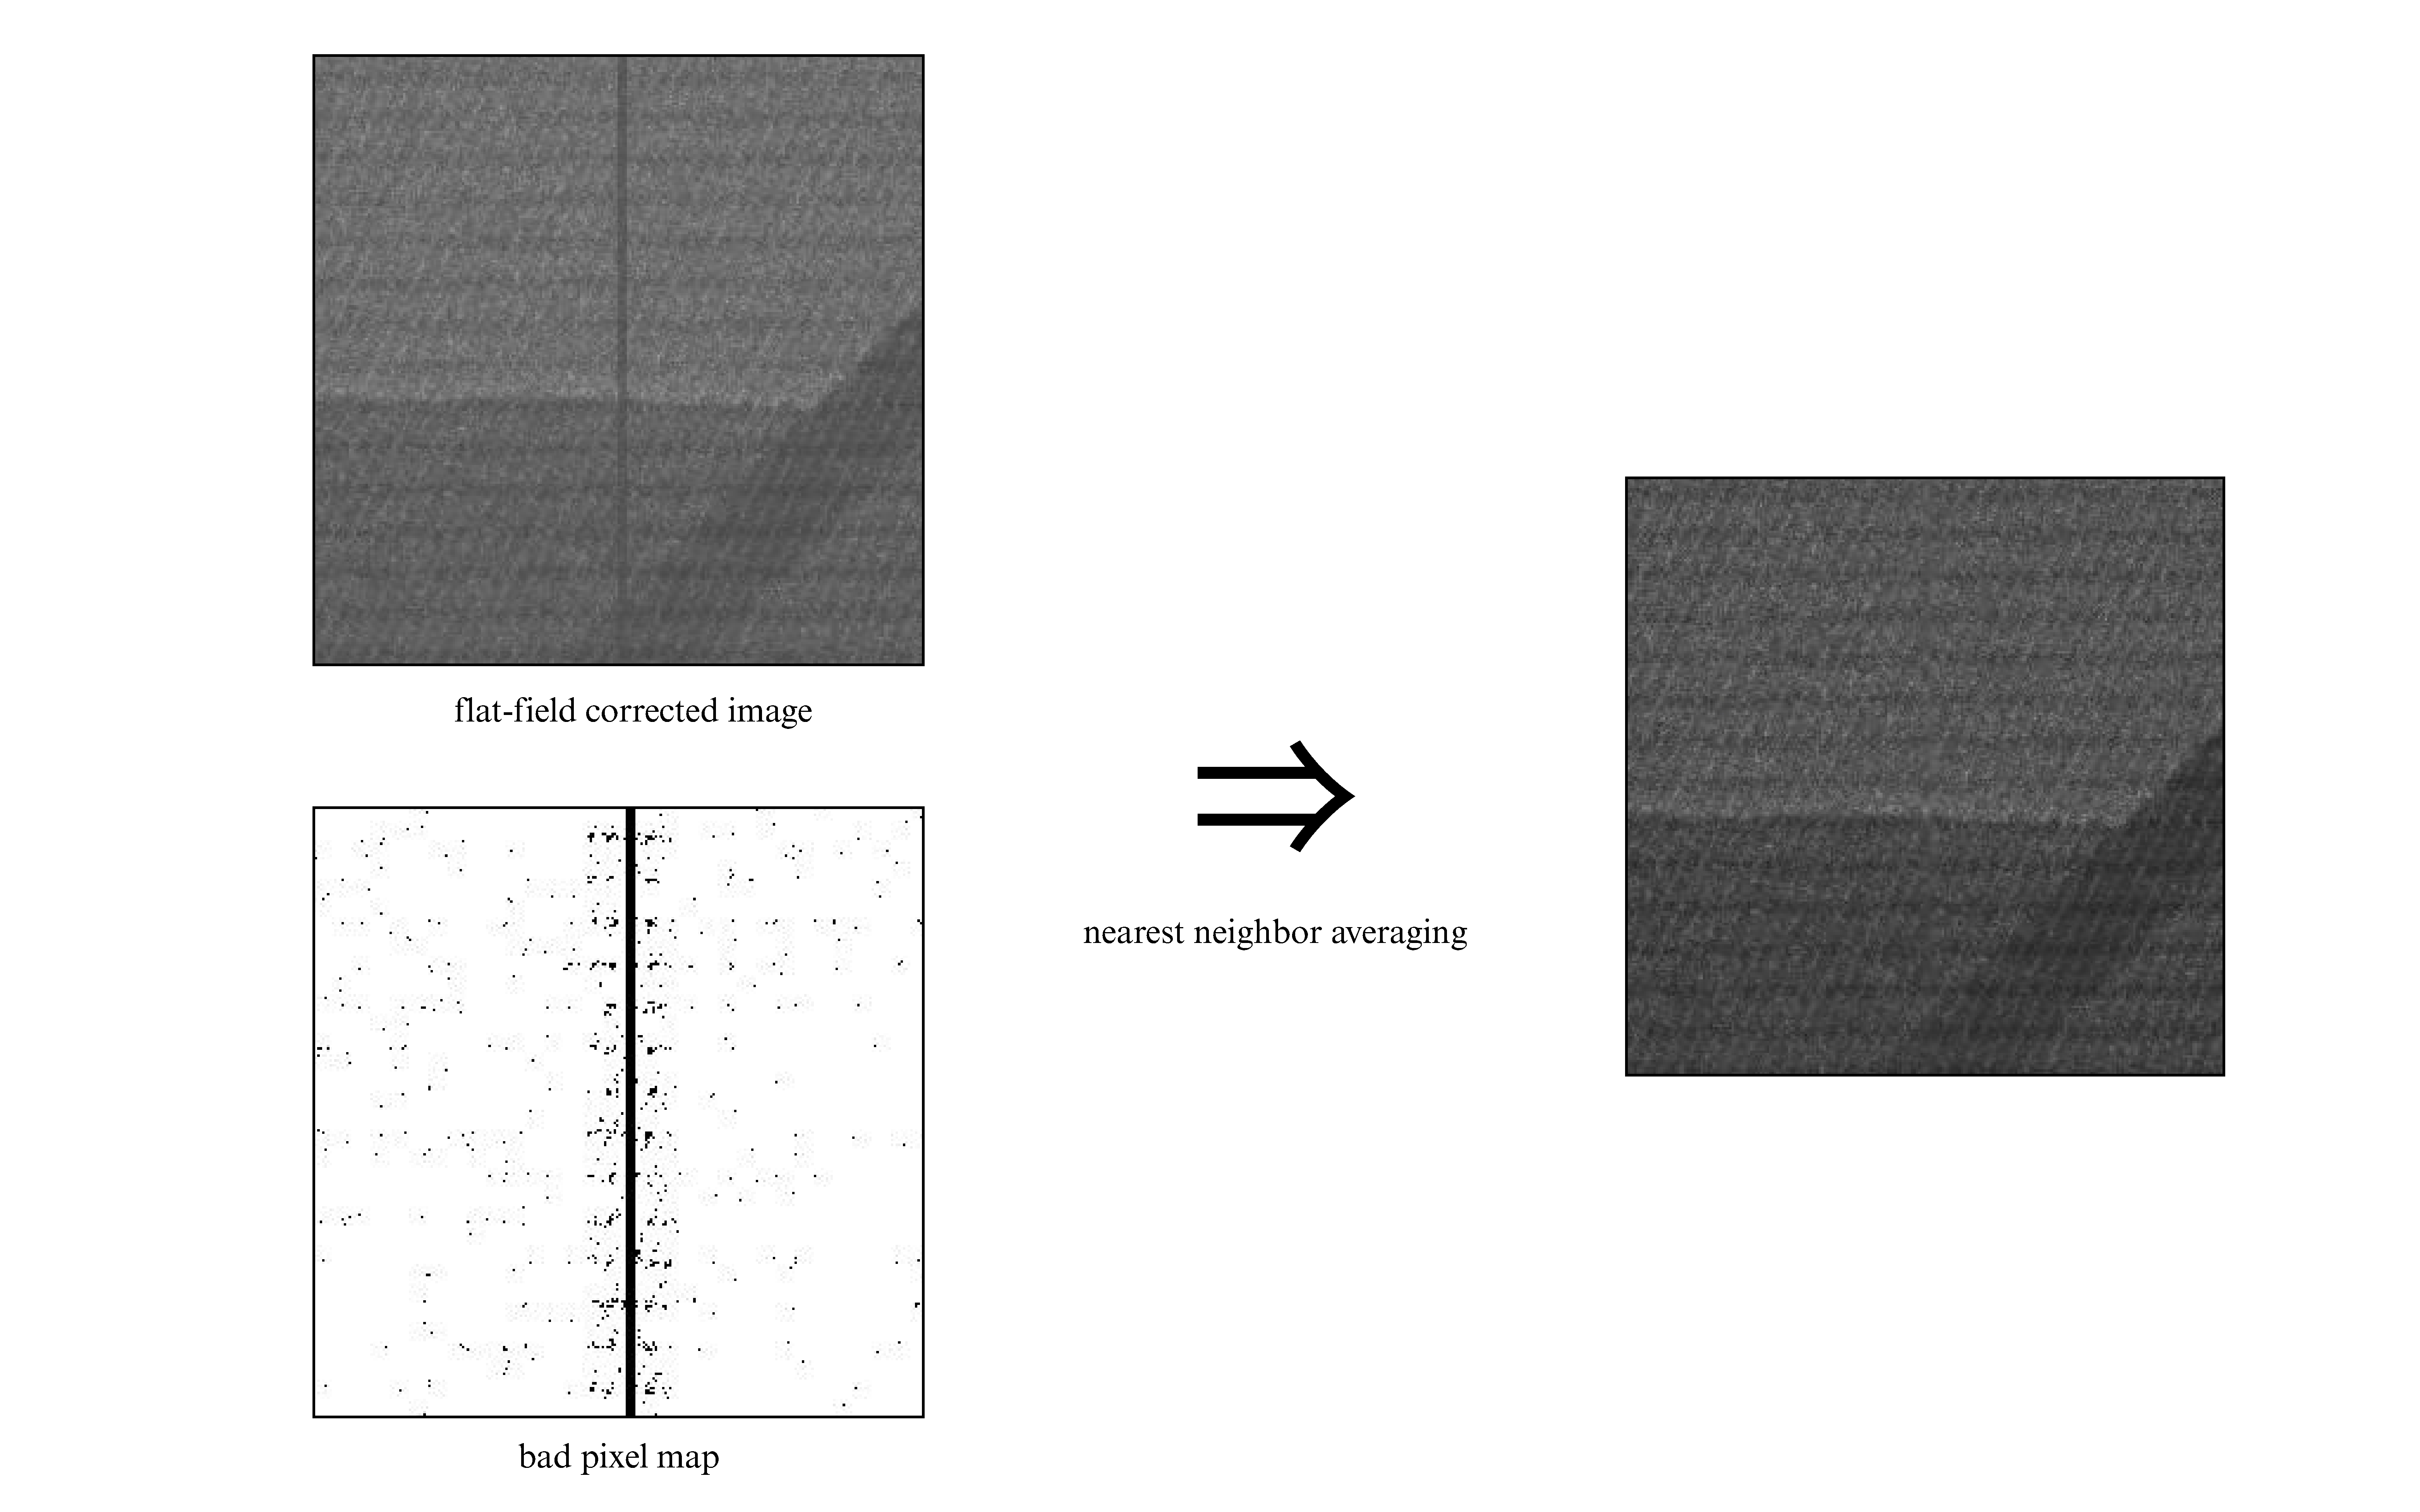
\includegraphics[width=0.85\textwidth, angle=0]{bad_pixel_correction.pdf}
 \caption{Bad pixel correction demonstration using bad pixel map}
 \label{fig:Bad pixel correction}
\end{figure}

\subsubsection{Fourier filtering}

Due to reasons such as glass between our source and the detector, horizontal and vertical streaks may appear in our frames. These streaks move and change position, phase, or frequency depending on the capture. The streaks are unwanted because they will cause streaking in the 3d reconstruction which aren't representative of the actual object scanned. \newline

To remove these streaks, the image must be analyzed in the frequency domain. Because the streaks are consistent, they appear as peaks in the Fourier domain. To view the images in the frequency, a 2d fast fourier transform or fft is applied. This is computationally less expensive compared to the normal discrete fourier transform and saves significant computation time due the large image size and quantity of images. \newline

In the frequency domain, the low frequency zone is very data dense and, whilst the higher frequency contains more noise. A decreasing gradient is also noticeable from the low frequencies to the higher frequencies. Because the low frequency area is data dense and has generally high values, a mask is applied to this area to make sure no changes are applied. \newline


Now, two values must be set: the peak mask size and the average mask size. The maximums are then found in this masked frequency domain. At each maximum, the mean and standard deviation are computed of the nearest neighbors with a kernel of size average mask size. A mask is created with the size of the peak mask size. This mask is filled is filled with gaussian noise based on the mean and standard deviation previously found. Even though the high frequencies are less data dense, due to the decreasing gradient and the need to keep the fidelity of the image, the mask should be representative of the area in which it is placed, therefore the need for the gaussian noise. The maximums are searched for until the limit set by the user. \newline

Once all the peaks are masked, the image is transformed back and the most significant streaks are removed (figure \ref{fig:Fourier Filtering Process}). Due to only a certain amount of peaks being removed, the borders still show some streaks, but because the borders aren't important to the reconstruction, it is a non-issue. 


\begin{figure}[h]
   \centering      
    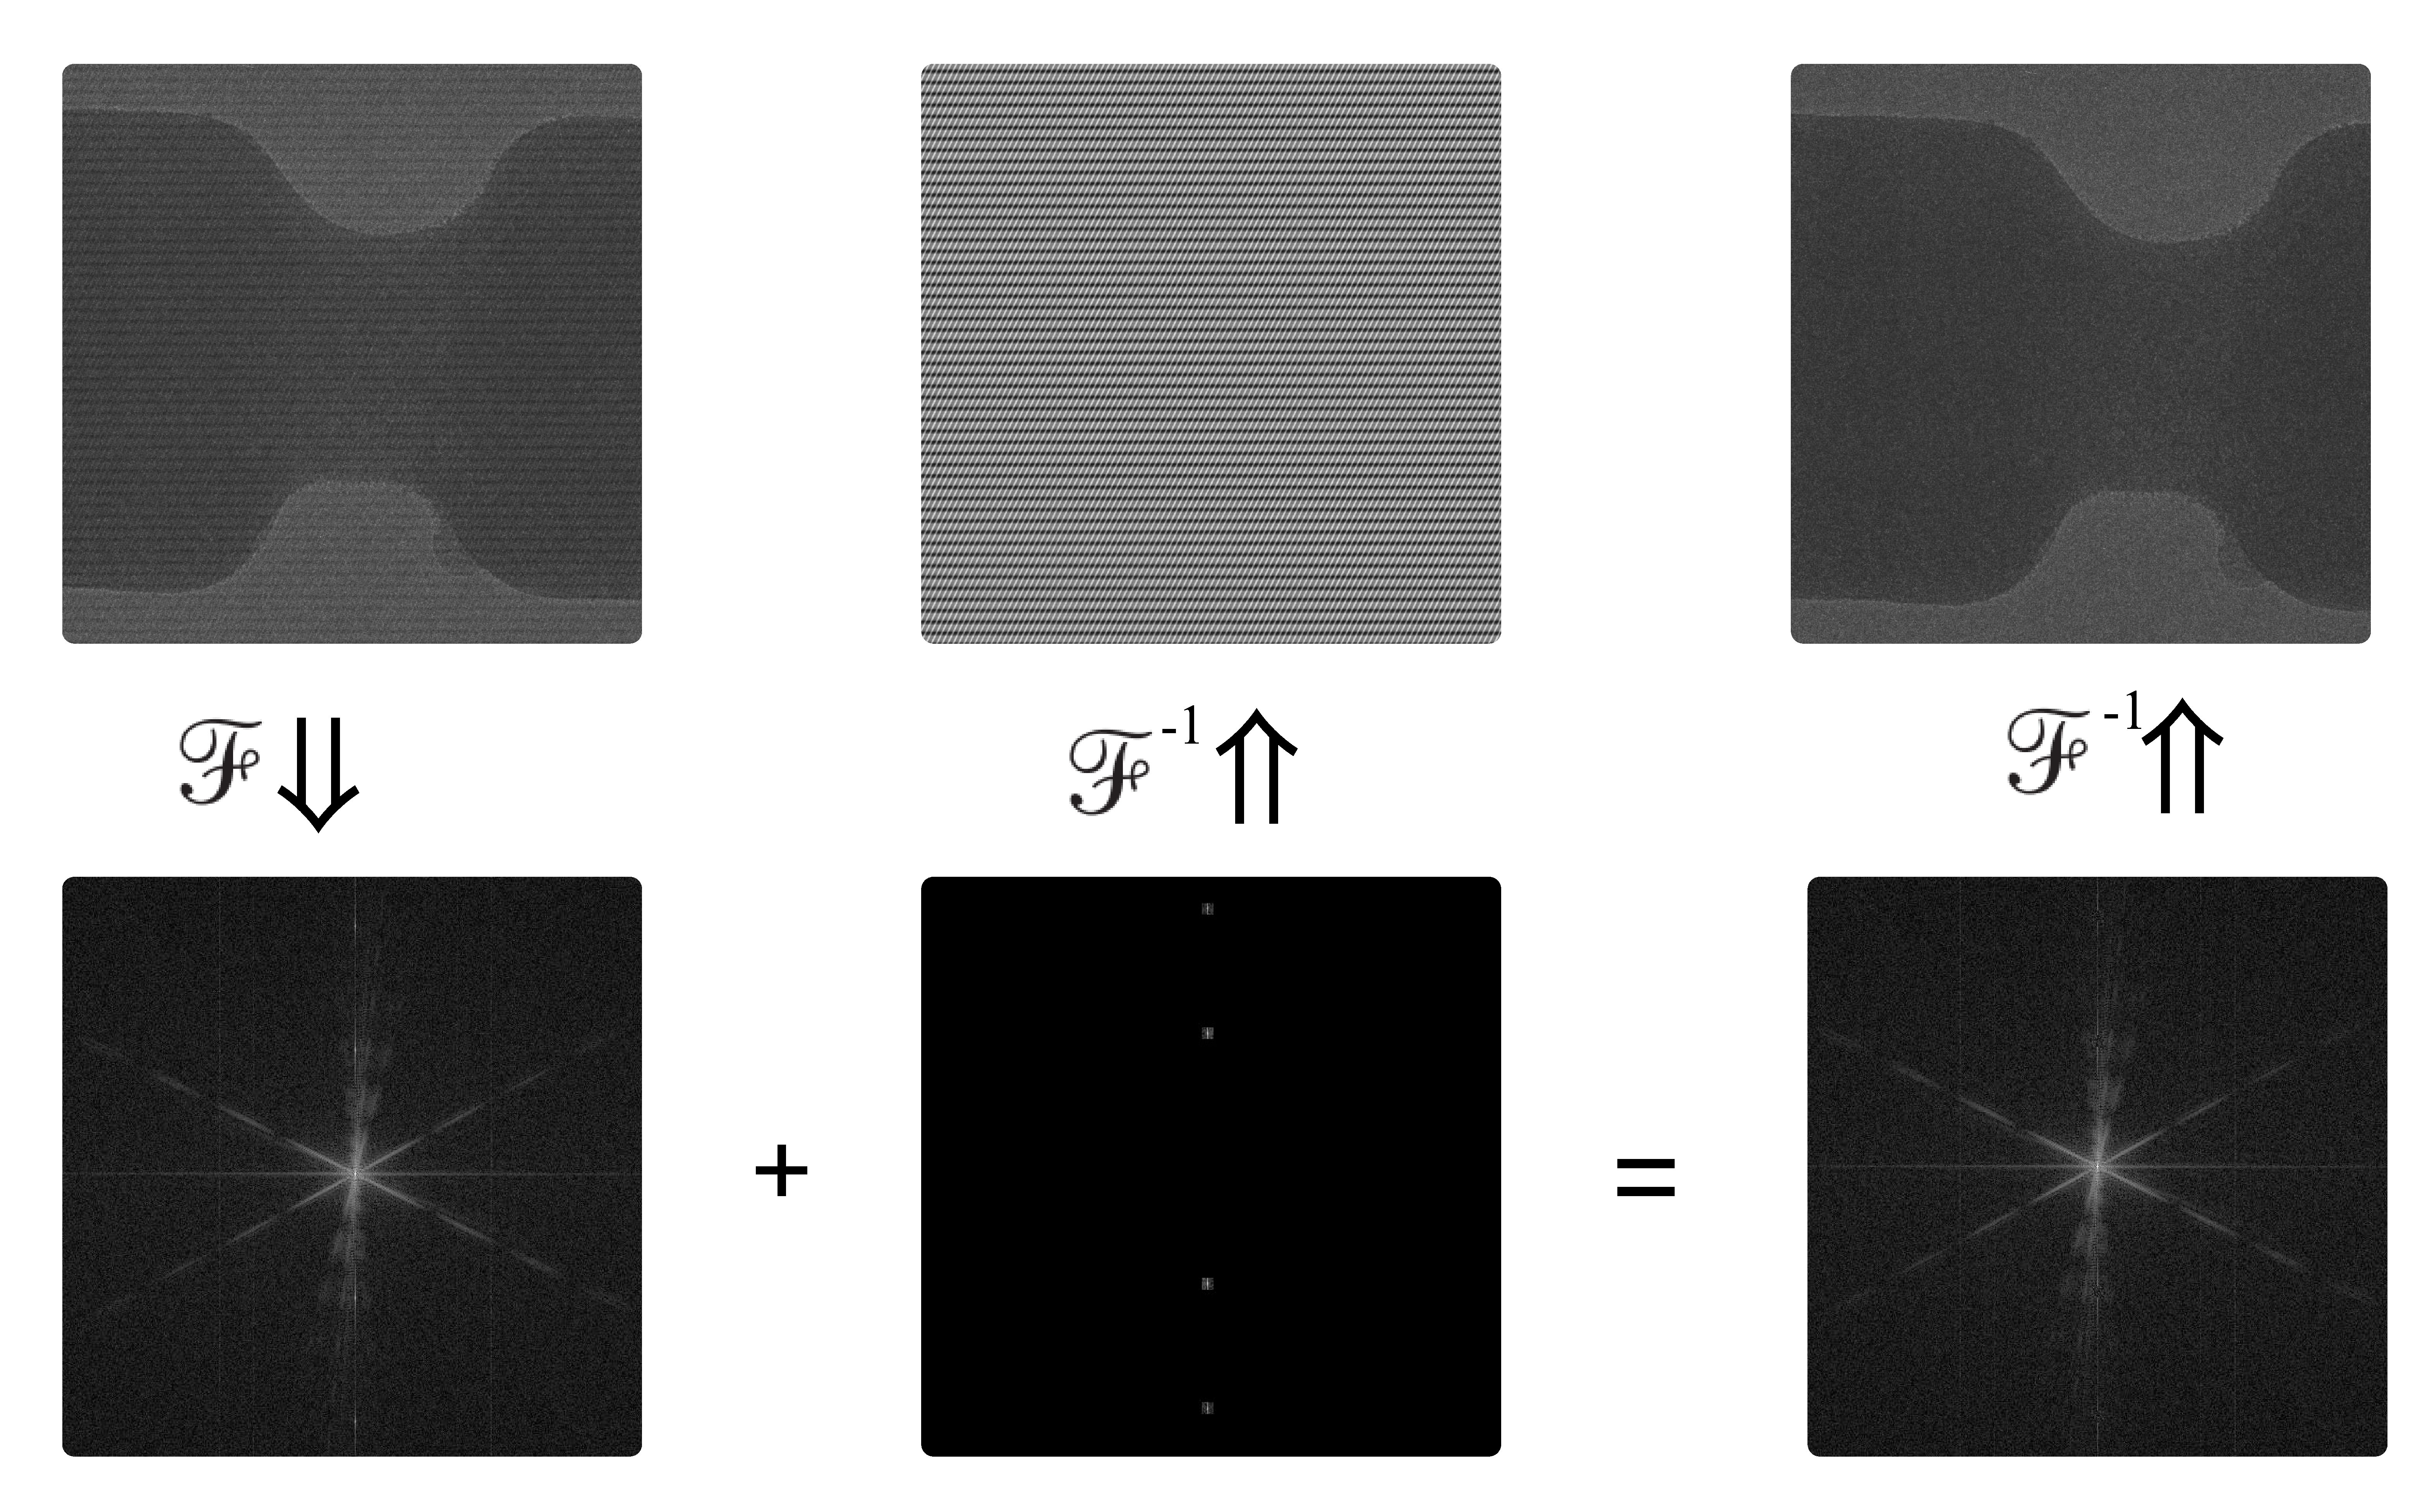
\includegraphics[width=1\textwidth, angle=0]{FourierFilteringProcess.pdf}
 \caption{Frequency domain processing pipeline}
 \label{fig:Fourier Filtering Process}
\end{figure}



\subsubsection{Image alignment}

The individual frames are not only inconsistent in terms of x-ray flux, but also in terms of position of the x-ray source. This means that from frame to frame, the captured object may appear to move up and down or side-to-side. \newline

To compensate, the phase correlation technique is applied. Normally phase correlation can be applied to images without any pre-processing, but due to the difference in flux and general noisiness of the frames, this can't be done. Before, some filters must be applied to the image to reduce the error caused by the noise and make the features of the object more apparent. \newline

For each frame, the extremes are clipped, meaning that pixel values farther from the mean than a certain threshold are clipped to that threshhold. Noise is still apparent, but the features are more visible. To remove the noise, a median filter is applied with a kernel size of 3. This is then normalized and rounded. The resulting image is black and white showing the features (figure \ref{fig:features}) and the image is cropped to show only part of the scanned object. \newline

With consistency across the frames, the phase correlation can be applied with each frame being compared to the first in the set.

% \[  \text{phase correlation formula } \]


\begin{figure}[h]
\centering
  \begin{subfigure}{.5\textwidth}
    \includegraphics[width=1\linewidth]{corrected_image_1.pdf}
  \end{subfigure}%
    \begin{subfigure}{.5\textwidth}

    \includegraphics[width=1\linewidth]{feature_corrected_image_1.pdf}
  \end{subfigure}%

    \caption{Comparison of image and image features}
    \label{fig:features}
\end{figure}



With the phase determined, the original non-clipped images are then shifted to their new positions. Most frames are aligned properly, but some exceptions may occur. To account for the exceptions, if the offset is too large, the frames are discarded.

\subsubsection{Averaging}

The final step is averaging the frames to obtain the projections. The projections are then normalized and inversed so that the higher valued pixel are the ones of the object. The tomographic scans are ready for reconstruction at this point.

\subsubsection{Multithreading}

Due to the time size and quantity of images, for each angle, the initial corrections for each frame, the flat-field, the bad pixel and the Fourier filtering, are done concurrently to reduce time. This time depends on the amount of available threads on the CPU.



\subsection{Reconstruction}

\subsubsection{Geometry}

For any tomographic reconstruction process, the geometric parameters must be well known. In most cases, such as with a spiral CT, these parameters are well defined because of the circular and constant nature of the scan. In the case of the ALLS betatron, these parameters are always subject to change. In addition to potentially differing parameters, the definition of the parameters are subject to change from software to software and from researcher to researcher.  Due to the modular nature of taking scans with the ALLS betatron, the parameters needed must be concise and consistent, yet sufficient for all possible scans. The objects in the geometry are the source, the detector, and the object. All parameters are defined in the reference frame of the source due to the physical measurements being taken from the source's reference frame.\newline 

The detector is defined as a 2d plane in the 3d space. It's length and width in pixels (the same size as the tomographic scans), the pixel size, the position of the center pixel in the reference frame of the source, and angles of the rows and columns of the detector. The cross product between the column vector and row vector is the face the detector receives the rays. Should it not be done properly, the reconstruction may be flipped. The object is defined as rectangular prism. The prism has a height, length and width in voxels, the voxel size, the position of the volume in the reference frame of the source and the angle of rotation.\newline 

All these parameters are converted to the modular-beam geometry in the LEAP open-source reconstruction library. 

\begin{table}[h!]
\caption{Geometry parameters which must be defined for proper and complete reconstruction} \label{tab:geometry_table}
\begin{tabular}{p{3.5cm}|p{1.5cm}|p{9cm}}
Parameter Name & Unit & Description \\
\hline
\texttt{source to object distance} & mm & distance from the source to center of the object volume as a 3 dimensional vector \((x,y,z)\) \\
\texttt{source to detector distance} & mm  & distance from the source to center of the detector plane as a 3 dimensional vector \((x,y,z)\)\\
\texttt{axis of rotation} & radians & axis which the volume rotates around represented as a 2d vector \((\phi,\theta)\) \\
\texttt{row vector} & radians & direction of the detector rows represented as a 2d vector \((\phi,\theta)\) \\
\texttt{column vector} & radians &  direction of the detector columns represented as a 2d vector \((\phi,\theta)\)  \\
\texttt{row count} & none  &  amount of pixel rows \\
\texttt{column count} & none  &  amount of pixel columns \\
\texttt{pixel size} & mm  &  length of one of the detector's pixels' sides\\
\texttt{voxel size} & mm  &  length of one of the volume's voxels' sides \\

\end{tabular}
\end{table}


\begin{figure}[h]
   \centering      
    \includegraphics[width=1\textwidth, angle=0]{drawing.pdf}
 \caption{Tomography geometry diagram}
 \label{fig:geometry1}
\end{figure}


\subsubsection{Memory, video memory and helper functions}

The LEAP reconstruction library defines the reconstruction volume and the tomographic scans both as 3d arrays of type float32. This is difficult to change due to most of the code's library being written in CUDA and float16 compatibility being quite rare in most contexts. The bottlenecks can appear in both normal and video memory. \newline

To calculate the amount of memory used, the calculation is


\[\text{memory used} = dim_1 \cdot dim_2 \cdot dim_3 \cdot 4\text{ bytes } \] 

where \(dim_i\) is the \(i^{th}\) dimension of the array. \newline

Upon analysis of the memory and video memory, the entire tomographic scan and the entire volume is stored on RAM and the entire volume is copied to the GPU and therefore the video RAM when the projections and back-projections are being performed. If the volume is too large, the program will crash due to there not being enough available memory. Two helper geometries have been added to combat these bottlenecks: volume magnification and the detector cropping (figure \ref{fig:geometry2}). \newline

\begin{figure}[h]
   \centering      
    \includegraphics[width=1\textwidth, angle=0]{drawing2.pdf}
 \caption{Helper geometry visualization}
 \label{fig:geometry2}
\end{figure}

The detector cropping allows selection of a certain area of the projections, crops and adjusts the internal geometry of the detector. This is useful for when only a certain part of the tomographic scan is useful for the reconstruction. The volume magnification allows a selection of the volume, modification the voxel size, and also automatically adjusts the volume's geometry. This allows for more precise reconstruction and less memory usage, but the chosen area must be chosen properly or else the reconstruction will fail. The selected volume must contain all parts of the object which are shown in the tomographic scans. \newline

The optimal steps to use these functions are the following: 

\begin{enumerate}
    \itemsep-0.5em 
    \item Define a lower resolution (larger voxel size) reconstruction volume
    \item Choose tomographic scan cropping area parameters
    \item Perform initial reconstruction
    \item Crop volume to only where the object appears
    \item Set the magnification resolution
    \item Perform final reconstruction
\end{enumerate}

By setting a lower initial resolution to the volume size and cropping it after an initial reconstruction reduces the total time taken and eliminates possibility of crashes from allocating too much memory. 

\subsubsection{Back-projection}

In spiral geometries, analytic back-projection algorithms, such as the inverse-radon transform, are effective. When the object does not spin around itself vertically and at the center of the projection, the analytic algorithms do not work. Because of the non-spiral geometry of the betatron x-ray, iterative back-projection algorithms are most optimal for the source. The SART algorithm is the algorithm of choice. \newline

Simultaneous Algebraic Reconstruction Technique or SART is an algorithm conceived by A. H. Andersen and A. C. Kak in 1984 as an upgraded version of the ART algorithm  created by Richard Gordon in 1970 due to the "salt and pepper" look ART results \cite{ANDERSEN198481,GORDON1970471}. Due to the complexity of the algorithm, it will not be explained.  





\subsection{Parameter Optimization} 

The general parameters of the reconstruction geometry that are measured in person during the scan are just an estimation. To obtain the most precision in the reconstruction, these parameters must optimized automatically. \newline

The simplest approach to optimizing these parameters is using machine learning. Most machine learning algorithms can be optimized using gradient descent because the function/neural networks being optimized are well defined analytically. The reconstruction algorithm is not defined analytically and can be considered a black box function. Therefore the parameters must be optimized using bayesian optimization which is tailored for black box functions. 

\subsubsection{Loss function}

The optimization algorithm alone doesn't ensure good parameter estimation. Thus, a good loss function must be chosen. The minimum of this function should be where the parameters are the most accurate. Should it not, the reconstruction will be innacurate depending on the loss function chosen. Initial tests were done with loss functions based on image gradients optimizing for sharpness and loss functions based on analyzing the pixel value spectrogram, but these arent the most optimal in all use cases. Because there is no reference for a reconstructed object, it's difficult to define a loss function based only this. The only references available are the initial tomographic scans. The reconstruction can be projected back to the tomographic scans and can be compared to the ones used for the reconstruction. \newline


\begin{figure}[h]
\centering
  \begin{subfigure}{.45\textwidth}
    \includegraphics[width=1\linewidth]{base_tomographic_scan.pdf}
    \caption{Initial tomographic scan}
  \end{subfigure}%
    \begin{subfigure}{.45\textwidth}

    \includegraphics[width=1\linewidth]{reprojection.pdf}
    \caption{Re-projected tomographic scan}
  \end{subfigure}%

    \caption{Example of tomographic scan and re-projected tomographic scan}
    \label{fig:diff1}
\end{figure}



\begin{figure}[h]
\centering
\includegraphics[width=0.65\linewidth]{loss_1.pdf}
\caption{First loss function}
    \label{fig:loss1}

\end{figure}


Two comparisons are done. A first comparison done is by simply taking the mean square error of the real and synthetic tomographic scans (figures \ref{fig:diff1} and \ref{fig:loss1}). In addition to this loss, a loss is taken with the extracted features. Like in the pre-processing for the phase correlation, the features are extracted leaving a black and white image showing the shape of the object (figures \ref{fig:diff2} and \ref{fig:loss2}). A mean squared error is then applied to the processed images making sure that the size of the reconstructed image isn't different. Summing these two error functions allows the bayesian optimization to find the reconstruction with not only the most similar shape to the original, but also the best sharpness and inner-feature reconstruction.





\begin{figure}[h]
\centering
  \begin{subfigure}{.45\textwidth}
    \includegraphics[width=1\linewidth]{img2.pdf}
    \caption{Initial tomographic scan features}
  \end{subfigure}%
    \begin{subfigure}{.45\textwidth}

    \includegraphics[width=1\linewidth]{img1.pdf}
    \caption{Re-projected tomographic scan features}
  \end{subfigure}%

    \caption{Example of calibration frames}
    \label{fig:diff2}
\end{figure}



\begin{figure}[h]
\centering
\includegraphics[width=0.65\linewidth]{loss_2.pdf}
\caption{Second loss function}
\label{fig:loss2}

\end{figure}






\clearpage
\section{Results}

\subsection{Image pre-processing}

The image pre-processing pipeline was tested on tomographic scans of an alloy rod. The major streaking issues are all accounted and the images are well-aligned. The resulting images are of high fidelity and the fine details of the rod. Without the alignment, the images end up flat and lack sharpness (figure \ref{fig:comparison}). \newline

\begin{figure}[h]
\centering
  \begin{subfigure}{0.5\textwidth}
    \includegraphics[width=1\linewidth]{zoomed_aligned.pdf}
    \caption{Aligned frames}
  \end{subfigure}%
    \begin{subfigure}{0.5\textwidth}

    \includegraphics[width=1\linewidth]{zoomed_unaligned.pdf}
    \caption{Unaligned frames}
  \end{subfigure}%

    \caption{Comparison of final tomographic scans with and without phase correlation}
    \label{fig:comparison}
\end{figure}

The time to correct all the images depends on the CPU of the computer used to perform the corrections. The most demanding part of the processing is performing many Fourier transforms and their inverses on thousands of images. In the case of the rod, there were 30 captures for 180 angles and each capture is unsigned int16 4096 by 2048 image. This results in 91 gigabytes of image. Initially, the pre-processing time took around 90 minutes. With multithreading, the time to complete the pre-processing ends up being around 33 minutes, or 11 seconds per angle, on an AMD Ryzen 5900x CPU. Figure \ref{fig:result1} shows a zoomed-in version of the final result where the detail can be seen.


\begin{figure}[h]
\centering
\includegraphics[width=0.9\linewidth]{zoomed.pdf}
\caption{Cropped version of final tomographic scan }
\label{fig:result1}

\end{figure}


\subsection{Computed Tomography}

\subsubsection{Memory, video memory and helper functions.}

The helper functions that reduce memory and video memory usage also work as needed and speed up reconstruction time. As mentioned previously, the volume cropping mechanism needs to be used carefully to avoid cropping any object features; if this happens, the entire volume turns black, meaning no object can be reconstructed. When used in combination properly following the steps explained previously, the time gains are immense. \newline


When tested with the projections phantom (figure \ref{fig:shepp_cropped} where the result wanted was the middle layers of the phantom, the time gain was of 500\%. Initially, with a full tomographic scan, with a SART reconstruction with 10 subsets and 10 iterations, the reconstruction time was of 104 seconds. After cropping the tomographic scan for the important area, cropping the volume and keeping the same SART reconstruction parameters, the elapsed time was of 20 seconds. 

\begin{figure}[h]
\centering
\includegraphics[width=0.8\linewidth]{cropping.pdf}
\caption{Cropping helper function used on tomographic scan of the shepp-logan phantom}
\label{fig:shepp_cropped}
\end{figure}

These helper functions reduced the memory usage from 69.20 megabytes to 16.98 megabytes. These values fit easily in memory, but when used on larger datasets, this will help the code not crash. 

\subsubsection{Initial reconstructions}


For the reconstruction of the rod, the only parameters known were the source to object distance and the source to detector distance which still just good estimates. The object rotated close to horizontally and the detector was more or less perpendicular to the incoming beams. This means it was the perfect scenario to use the parameter optimization process. There were 180 angles and each frame was 4096x2048 pixels with each pixel being uint16. This comes out to 6.03 gigabytes. Depending on the precision wanted from the reconstruction, the reconstruction volume could vary from 536 megabytes to 274 gigabytes. The latter is unreasonably large and can't fit on any GPU. This was therefore also the perfect opportunity to use the helper geometries to reduce both the tomographic scans and the volume size. The initial parameters were: \newline

\begin{table}[h!]
\centering

\caption{Initial geometry parameters for the alloy rod} \label{tab:geometry_table}
\begin{tabular}{p{4cm}|p{4cm}|p{4cm}}
Parameter Name & Unit & Values \\
\hline
\texttt{source to object distance} & mm & \((0,775,0)\) \\
\texttt{source to detector distance} & mm  & \((0,2360,0)\)\\
\texttt{axis of rotation} & radians & \((0,0)\) \\
\texttt{row vector} & radians &  \((-\pi/2,0)\) \\
\texttt{column vector} & radians &  \((0,0)\)  \\
\texttt{pixel size} & mm  &  \(0.008\)\\

\end{tabular}
\end{table}

Without using any of the helper geometries or any parameter optimization, the initial results showed the object without any major physical defects, but had low contrast and couldn't show any of the inner features (figure \ref{fig:comparison_i_reconstruction} (a)). The full tomographic scans contain alot darkness and if the SART parameters are adjusted for this, the results won't be clear. However, by adjusting the parameters to compensate, the reconstructions will take significantly longer. Having the shape of the whole rod was not the goal. The goal was to be able to view the pores within the indented section of the rod. The helper geometries facilitated thi. The tomographic scans were cropped where the indented section is fully visible at all times for each angle. \newline

% \begin{figure}[h]
% \centering
% \includegraphics[width=0.5\linewidth]{whole_reconstruction.pdf}
% \caption{Initial full reconstruction of the alloy rod}
% \label{fig:whole_recon}
% \end{figure}

\begin{figure}[h]
\centering
\includegraphics[width=0.1\linewidth]{cropped_for_geom.pdf}
\caption{Alloy rod cropped with geometry helper functions}
\label{fig:rod_cropped}
\end{figure}


\begin{figure}[h]
\centering
  \begin{subfigure}{0.4\textwidth}
    \includegraphics[width=1\linewidth]{whole_reconstruction.pdf}
    \caption{Uncropped tomographic scan}
  \end{subfigure}%
    \begin{subfigure}{0.4\textwidth}
    \includegraphics[width=1\linewidth]{test-1.pdf}
    \caption{Cropped tomographic scan}
  \end{subfigure}%
    \caption{Comparison of the reconstruction with the initial parameters before and after cropping the tomographic scan}
    \label{fig:comparison_i_reconstruction}
\end{figure}


The results with the reduced tomographic scans (figure \ref{fig:rod_cropped} (b)) are much better contrast (figure \ref{fig:comparison_i_reconstruction} (b)). The tomographic scan cropping reduced the RAM usage for the projections from 6 gigabytes down to 490 megabytes. This creates a speed-up but also allows the reconstruction to be run on lower-end machines. The pores are naturally visible when zoomed to without having to adjust the contrast. Black bars appear on the reconstruction volume. This is where the SART algorithm didn't have enough information from the tomographic scans to complete the reconstruction of the areas. These volumes can be cropped later on with the helper geometries. Spherical artifacts appears in the reconstruction in cuts of the x-axis; this is due to the axis of rotation being perpendicular to that axis (figure \ref{fig:all_3}). If the contrast is adjusted, the pores become very visible figure \ref{fig:all_3_contrast}). 

\begin{figure}[h]
\centering
\includegraphics[width=0.85\linewidth]{no_contrast_3.pdf}
\caption{Example of cuts int each axis of the reconstructed object after using the helper geometries}
\label{fig:all_3}

\end{figure}

\begin{figure}[h]
\centering
\includegraphics[width=1\linewidth]{contrast_3.pdf}
\caption{Example of cuts int each axis of the reconstructed object after using the helper geometries and adjusting for contrast}
\label{fig:all_3_contrast}

\end{figure}

\section{Discussion}
\subsection{Difficulties}

Although there weren't many difficulties that arose during the development process, the ones that did caused major issues. The first that was run into was the need for CUDA. Most tomographic reconstruction software that is reasonably high-performance utilizes CUDA cores to accelerate the reconstruction process because of the need for parallelization. The ones that didn't were restricted to simple spiral geometries or incredibly slow. The only option was to use CUDA. The choice of software/library was not immediate either. There are a vast amount, but the most complete and still open-source option was LEAP. The second major issue was learning how to use the LEAP library and appropriate it for the betatron X-ray. It took some time to create a geometry that reduced the amount of parameters enough to reduce the amount of parameters needed in the Gaussian process. The third and final major issue was dealing with the memory in an appropriate way. Some of my initial tactics like trying to modify the source code use float16 instead of float32 failed and I resorted to creating the helper geometry which ended up helping debugging later on.





\subsection{Recommendations and future work}

Even though the projections obtained after the pre-processing allow good reconstructions, there are some changes which can be done to enhance the projections.

\subsubsection{Fourier filtering}

The streak removal processing by filtering in the Fourier domain yields good results, but the approach explained and used is naive and primitive. \newline

\begin{figure}[h]
   \centering      
    \includegraphics[width=0.4\textwidth, angle=0]{completed_flipped_noclipped_aligned_cropped.pdf}
 \caption{Streak removal process artifacts}
 \label{fig:Streak removal process artifacts}
\end{figure}

As seen in figure \ref{fig:Streak removal process artifacts}, the process creates streaks near the top of the image and across some diagonals. This can be due to removing peaks in the Fourier which represent important data, but weren't contained in the initial masked because they are considered higher frequency, can be due to the masking approach used to cover the peaks or due to the data loss from performing a the Fast Fourier Transform and inverting it back to the real domain. \newline

\begin{figure}[h]
   \centering      
    \includegraphics[width=0.8\textwidth, angle=0]{zoom_in_fourier.pdf}
 \caption{Fourier domain zoom-in to peak}
 \label{fig:Zoom}
\end{figure}

Visible in figure \ref{fig:Zoom}, each peak that would eventually be suppressed has two features which aren't accounted for: vertical streaks and sub-peaks horizontal to the main peaks. Due to the naive masking of the main peaks (figure \ref{fig:Before and after fourier filtering}), the sub-peaks, which have amplitudes that are smaller than the main peaks, but larger than the background noise, won't ever be masked. The vertical streaks, which have larger values than the average noise behind, also won't be masked.
\newline


\begin{figure}[h]
\centering
  \begin{subfigure}{.5\textwidth}
    \includegraphics[width=1\linewidth]{0.pdf}

            \caption{before}

  \end{subfigure}%
    \begin{subfigure}{.5\textwidth}

    \includegraphics[width=1\linewidth]{14.pdf}
        \caption{after}

  \end{subfigure}%

    \caption{Before and after fourier filtering}
    \label{fig:Before and after fourier filtering}
\end{figure}


An easy approach would be to mask a larger area, but to reduce data loss, this isn't recommended. To fix the issues of the sub-peaks not being masked, for a certain distance away from the main peaks, simply perform a simple search to the left and right of the main peak for values which are 1 or 2 standard deviations larger than the mean of the local area. To fix the streaks, a gradient descent would be optimal; starting from the peak, follow the gradient in y and suppress until the pixel  reached is within 1 standard deviation of the local pixel value mean.

\subsubsection{Image alignment}

The approach used for aligning the different frames of the same angle is less naive than the fourier filtering, but has its drawbacks too. \newline

As previously mentioned in the methodology, images' whose corrected shift were clearly unusual were discarded. This was done because for some unknown reason, for certain frames of the same shot, the shift was too large and caused bad averages. Because 30 shots were taken per angle, a few being discarded doesn't really cause a large difference. If one wanted to fix this, it's really a matter of finding a feature extraction process that reduces the amount shots discarded. \newline

All the images were aligned to the first of the set, which is arbitrary. A better way would be to first take the average of all the frames. Calculate the phase difference between the frames and the average. The frame that has the smallest shift would then be considered the base. All the other frames of the set would then be aligned to the base. 

\subsubsection{Parameters optimization} 

Humans are able to differentiate between clear and non-clear reconstructions and it is difficult to quantify this clearness, especially in a voxelized space. Instead of re-projecting the reconstructions and comparing them to the original scans, it would be interesting to develop a CNN-based no-reference image quality metric trained on a custom dataset. This dataset would be created by finding a dataset of 3d models, voxelizing them, projecting them and then re-projecting them with a different geometry. The loss would be the difference between the original voxel model and the faulty re-projection. This has been done on images by Kamal Lamichhane and has an interesting potential in this situation \cite{LAMICHHANE2023116899}.


\section{Conclusion}

In conclusion, betatron tomography via laser Wakefield acceleration demonstrates very promising results. With enough image pre-processing, tomographic scans obtained through these x-rays are of high quality. Using the CUDA powered library LEAP, reconstructing the objects is done quickly which allows for extensive debugging without having to wait substantially unlike non GPU-accelerated tomographic reconstruction libraries. With Bayesian optimization, initial parameters can be optimized to yield the best possible reconstructions. 

\clearpage
\section{Appendix}

\subsection{Installation guide}

The code written is based on the library LEAP by the Lawrence Livermore National Laboratory. Additional libraries such as numpy, tamari, scipy, scikit-image were used as well. The code is hosted at \url{https://github.com/INRS-EMT-ALLS/TomoALLS}. To clone the repository, make sure git is installed and run \verb| git clone https://github.com/INRS-EMT-ALLS/TomoALLS.git|. The file structure will be the following: \newline

\dirtree{%
.1 TomoALLS.
.2 src.
.3 projection\_io.py.
.3 projection\_visualization.py.
.3 projection\_preprocessing.py.
.3 projection\_reconstruction.py.
.2 examples.
.3 import\_pipeline.py.
.3 view\_corrected.py.
.3 rod\_reconstruction.py.
.3 crop\_tomographic scans.py.
.2 requirements.txt.
.2 install.sh.
}
\vspace{5mm}

Following this, it is suggested to install all dependencies in a virtual environment. To do so, simply open a terminal in the \verb| TomoALLS| folder and run \verb|python -m venv .|. This creates a separate environment for all your python libraries and abstracts TomoALLS away from all other maybe problematic python libraries. To call python from this virtual environment, instead of running \verb|python main.py| in terminal, run \verb|bin/python main.py|. To install all the dependencies, the final step is to run \verb|install.sh| which is a bash script to install the LEAP library and all the python libraries needed. 

\subsection{Code library}

There are two main sections to the code library as seen in the file hierarchy: \verb|src| and \verb|examples|. If you only need to use the reconstruction and the pre-processing, everything you need is in the \verb|examples| folder. Should you want to modify any of the main source code, everything contained is in \verb|src|. 

\subsection{Source code}

The \verb|src| contains four source files: one for IO, one for visualization, one for pre-processing and one for reconstruction.

\subsubsection*{Projection IO}

All the input and output functions are in the \verb|projection_io.py| file. This includes batch import, exporting and exporting to jpeg.

\begin{verbatim}TomoALLS.src.projection_io.image_importer(path,height,width,dtype=np.uint16)
\end{verbatim}
\begin{adjustwidth}{1cm}{}
    This function imports a single \verb|.raw| file returns a 2d numpy array.\\
    \textbf{Parameters}
    \begin{adjustwidth}{1cm}{}
        \textbf{path}
            \begin{adjustwidth}{0.5cm}{}
            [string] Path of the \verb|.raw| projection to import
            \end{adjustwidth}
        \textbf{height}
            \begin{adjustwidth}{0.5cm}{}
            [int] Height of the image
            \end{adjustwidth}
        \textbf{width}
            \begin{adjustwidth}{0.5cm}{}
                [int] Width of the image
            \end{adjustwidth}
        \textbf{dtype}
            \begin{adjustwidth}{0.5cm}{}
            [dtype, optional] Datatype of the \verb|.raw| projection
            \end{adjustwidth}
    \end{adjustwidth}
    \textbf{Return}
    \begin{adjustwidth}{1cm}{}
        \textbf{out}
            \begin{adjustwidth}{0.5cm}{}
            [np.array] Projection as a 2d float32 np.array
            \end{adjustwidth}
    \end{adjustwidth}
\end{adjustwidth}

\begin{verbatim}TomoALLS.src.projection_io.directory_images_importer(dir,height,width,dtype=np.uint16)
\end{verbatim}
\begin{adjustwidth}{1cm}{}
    This function batch imports all \verb|.raw|s in a folder. \\
    \textbf{Parameters}
    \begin{adjustwidth}{1cm}{}
        \textbf{dir}
            \begin{adjustwidth}{0.5cm}{}
            [string] Directory of the \verb|.raw| projections to import
            \end{adjustwidth}
        \textbf{height}
            \begin{adjustwidth}{0.5cm}{}
            [int] Height of the images
            \end{adjustwidth}
        \textbf{width}
            \begin{adjustwidth}{0.5cm}{}
                [int] Width of the images
            \end{adjustwidth}
        \textbf{dtype}
            \begin{adjustwidth}{0.5cm}{}
            [dtype, optional] Datatype of the \verb|.raw| projection
            \end{adjustwidth}
    \end{adjustwidth}
    \textbf{Return}
    \begin{adjustwidth}{1cm}{}
        \textbf{out}
            \begin{adjustwidth}{0.5cm}{}
            [np.array] Projection as a 3d float32 np.array
            \end{adjustwidth}
    \end{adjustwidth}
\end{adjustwidth}

\begin{verbatim}TomoALLS.src.projection_io.image_exporter(image, path ,dtype=np.uint16)
\end{verbatim}
\begin{adjustwidth}{1cm}{}
    This function exports a projection to a  \verb|.raw| to be used later\\
    \textbf{Parameters}
    \begin{adjustwidth}{1cm}{}
        \textbf{image}
            \begin{adjustwidth}{0.5cm}{}
            [np.array] 2d greyscale np.array that will be converted back to a \verb|.raw| file
            \end{adjustwidth}
        \textbf{path}
            \begin{adjustwidth}{0.5cm}{}
            [string] Path of the \verb|.raw| which the image will exported to 
            \end{adjustwidth}
        \textbf{dtype}
            \begin{adjustwidth}{0.5cm}{}
            [dtype, optional] Datatype of the \verb|.raw| projection
            \end{adjustwidth}
    \end{adjustwidth}
\end{adjustwidth}

\begin{verbatim}TomoALLS.src.projection_io.image_to_jpeg(image, path ,dtype=np.uint16)
\end{verbatim}
\begin{adjustwidth}{1cm}{}
    This function exports a projection to a  \verb|.jpeg| to be viewed later \\
    \textbf{Parameters}
    \begin{adjustwidth}{1cm}{}
        \textbf{image}
            \begin{adjustwidth}{0.5cm}{}
            [np.array] 2d greyscale np.array that will be converted back to a \verb|.jpeg| file to be able to be viewed
            \end{adjustwidth}
        \textbf{path}
            \begin{adjustwidth}{0.5cm}{}
            [string] Path of the \verb|.jpeg| which the image will exported to 
            \end{adjustwidth}
        \textbf{dtype}
            \begin{adjustwidth}{0.5cm}{}
            [dtype, optional] Datatype of the projection
            \end{adjustwidth}
    \end{adjustwidth}
\end{adjustwidth}



\subsubsection*{Projection visualization}

All the visualization tools are in the \verb|projection_visualization.py| file. These mainly use the napari library to display.


\begin{verbatim}TomoALLS.src.projection_visualization.viewer(images)
\end{verbatim}
\begin{adjustwidth}{1cm}{}
    This function displays with napari a sequence of images\\
    \textbf{Parameters}
    \begin{adjustwidth}{1cm}{}
        \textbf{images}
            \begin{adjustwidth}{0.5cm}{}
            [np.array] 3d np.array of the projections to be displayed
            \end{adjustwidth}
    \end{adjustwidth}
\end{adjustwidth}


\begin{verbatim}TomoALLS.src.projection_visualization.fft_viewer(images)
\end{verbatim}
\begin{adjustwidth}{1cm}{}
    This function displays with napari the fourier transforms of a sequence of images (it applies the fourier transform to each image) \\
    \textbf{Parameters}
    \begin{adjustwidth}{1cm}{}
        \textbf{images}
            \begin{adjustwidth}{0.5cm}{}
            [np.array] 3d np.array of the projections to be fourier transformed and displayed
            \end{adjustwidth}
    \end{adjustwidth}
\end{adjustwidth}

\subsubsection*{Projection pre-processing}

All the image processing functions are in the \verb|projection_preprocessing.py| file. This includes all the techniques mentioned in the methodology and more (helper functions, etc.).

\begin{verbatim}TomoALLS.src.projection_preprocessing.projection_correction(images,gain_map,
offset_map, bad_pixel_map,min_x,max_x,min_y,max_y)
\end{verbatim}
\begin{adjustwidth}{1cm}{}
    This function takes in all necessary maps and sub-projections for a single projection angle and applies the corrections and uses concurrency when possible\\
    \textbf{Parameters}
    \begin{adjustwidth}{1cm}{}
        \textbf{images}
            \begin{adjustwidth}{0.5cm}{}
            [np.array] 3d np.array containing every sub-projection for a single angle
            \end{adjustwidth}
        \textbf{gain\_map}
            \begin{adjustwidth}{0.5cm}{}
            [np.array] Gain map used in the gain correction
            \end{adjustwidth}
        \textbf{offset\_map}
            \begin{adjustwidth}{0.5cm}{}
                [np.array] Offset map used in the gain correction
            \end{adjustwidth}
        \textbf{bad\_pixel\_map}
            \begin{adjustwidth}{0.5cm}{}
            [np.array] Bad pixel map used in the bad pixel correction
            \end{adjustwidth}
        \textbf{min\_x}
            \begin{adjustwidth}{0.5cm}{}
            [int] Smaller x coordinate used when cropping the image for the image alignment 
            \end{adjustwidth}
        \textbf{max\_x}
            \begin{adjustwidth}{0.5cm}{}
            [int] Larger x coordinate used when cropping the image for the image alignment 
            \end{adjustwidth}
        \textbf{min\_y}
            \begin{adjustwidth}{0.5cm}{}
            [int] Smaller y coordinate used when cropping the image for the image alignment 
            \end{adjustwidth}
        \textbf{max\_y}
            \begin{adjustwidth}{0.5cm}{}
            [int] Larger y coordinate used when cropping the image for the image alignment 
            \end{adjustwidth}
    \end{adjustwidth}
    \textbf{Return}
    \begin{adjustwidth}{1cm}{}
        \textbf{out}
            \begin{adjustwidth}{0.5cm}{}
            [np.array] Final corrected projection as a 2d float 32 np.array
            \end{adjustwidth}
    \end{adjustwidth}
\end{adjustwidth}

\begin{verbatim}TomoALLS.src.projection_preprocessing.single_image_correction(images,gain_map,
offset_map, bad_pixel_map)
\end{verbatim}
\begin{adjustwidth}{1cm}{}
    This function applies the corrections which don't depend on the other sub-projections. It is used to speed up the total correction time by being the function called during concurrency\\
    \textbf{Parameters}
    \begin{adjustwidth}{1cm}{}
        \textbf{images}
            \begin{adjustwidth}{0.5cm}{}
            [np.array] 3d np.array containing every sub-projection for a single angle
            \end{adjustwidth}
        \textbf{gain\_map}
            \begin{adjustwidth}{0.5cm}{}
            [np.array] Gain map used in the gain correction
            \end{adjustwidth}
        \textbf{offset\_map}
            \begin{adjustwidth}{0.5cm}{}
                [np.array] Offset map used in the gain correction
            \end{adjustwidth}
        \textbf{bad\_pixel\_map}
            \begin{adjustwidth}{0.5cm}{}
            [np.array] Bad pixel map used in the bad pixel correction
            \end{adjustwidth}
    \end{adjustwidth}
    \textbf{Return}
    \begin{adjustwidth}{1cm}{}
        \textbf{out}
            \begin{adjustwidth}{0.5cm}{}
            [np.array] Corrected sub-projection as a 2d float 32 np.array
            \end{adjustwidth}
    \end{adjustwidth}
\end{adjustwidth}

\begin{verbatim}TomoALLS.src.projection_preprocessing.generate_bad_pixel_map(path,height,
width, kernel_size, dtype=np.uint16)
\end{verbatim}
\begin{adjustwidth}{1cm}{}
    This function generates the bad pixel map from a set of gain frames or from a gain map using the algorithm described in the methodology. It takes the average of the gain frames or directly the gain map. Applies a blur with OpenCV2 with the blur size being the kernel size. Finds the ratios and generates the bad pixel map.  \\
    \textbf{Parameters}
    \begin{adjustwidth}{1cm}{}
        \textbf{path}
            \begin{adjustwidth}{0.5cm}{}
            [string] Path of the gain frames used in the generation of the bad pixel map
            \end{adjustwidth}
        \textbf{height}
            \begin{adjustwidth}{0.5cm}{}
            [int] Height of the projection
            \end{adjustwidth}
        \textbf{width}
            \begin{adjustwidth}{0.5cm}{}
                [int] Width of the projection
            \end{adjustwidth}
        \textbf{kernel\_size}
            \begin{adjustwidth}{0.5cm}{}
            [np.array] Size of kernel used in the algorithm
            \end{adjustwidth}
        \textbf{ration}
            \begin{adjustwidth}{0.5cm}{}
            [float32] Ratio between the average map and the convoluted map's pixel at which they are considered bad pixels
            \end{adjustwidth}
    \end{adjustwidth}
    \textbf{Return}
    \begin{adjustwidth}{1cm}{}
        \textbf{out}
            \begin{adjustwidth}{0.5cm}{}
            [np.array] Bad pixel map as a 2d np.array
            \end{adjustwidth}
    \end{adjustwidth}
\end{adjustwidth}

\begin{verbatim}TomoALLS.src.projection_preprocessing.generate_offset_map(path,height, 
width, dtype=np.uint16)
\end{verbatim}
\begin{adjustwidth}{1cm}{}
    This function generates the offset map from a set of offset frames or directly imports the offset map  \\
    \textbf{Parameters}
    \begin{adjustwidth}{1cm}{}
        \textbf{path}
            \begin{adjustwidth}{0.5cm}{}
            [string] Path of the offset frames folder or the offset map
            \end{adjustwidth}
        \textbf{height}
            \begin{adjustwidth}{0.5cm}{}
            [int] Height of the projection
            \end{adjustwidth}
        \textbf{width}
            \begin{adjustwidth}{0.5cm}{}
                [int] Width of the projection
            \end{adjustwidth}
    \end{adjustwidth}
    \textbf{Return}
    \begin{adjustwidth}{1cm}{}
        \textbf{out}
            \begin{adjustwidth}{0.5cm}{}
            [np.array] Offset map as a 2d np.array
            \end{adjustwidth}
    \end{adjustwidth}
\end{adjustwidth}

\begin{verbatim}TomoALLS.src.projection_preprocessing.generate_gain_map(path,height, 
width, dtype=np.uint16)
\end{verbatim}
\begin{adjustwidth}{1cm}{}
    This function generates the gain map from a set of gain frames or directly imports the gain map  \\
    \textbf{Parameters}
    \begin{adjustwidth}{1cm}{}
        \textbf{path}
            \begin{adjustwidth}{0.5cm}{}
            [string] Path of the gain frames folder or the gain map
            \end{adjustwidth}
        \textbf{height}
            \begin{adjustwidth}{0.5cm}{}
            [int] Height of the projection
            \end{adjustwidth}
        \textbf{width}
            \begin{adjustwidth}{0.5cm}{}
                [int] Width of the projection
            \end{adjustwidth}
    \end{adjustwidth}
    \textbf{Return}
    \begin{adjustwidth}{1cm}{}
        \textbf{out}
            \begin{adjustwidth}{0.5cm}{}
            [np.array] Gain map as a 2d np.array
            \end{adjustwidth}
    \end{adjustwidth}
\end{adjustwidth}

\begin{verbatim}TomoALLS.src.projection_preprocessing.normalize(image)
\end{verbatim}
\begin{adjustwidth}{1cm}{}
    This function normalizes the input image between 0 and 1  \\
    \textbf{Parameters}
    \begin{adjustwidth}{1cm}{}
        \textbf{image}
            \begin{adjustwidth}{0.5cm}{}
            [np.array] Image to be normalized
            \end{adjustwidth}
    \end{adjustwidth}
    \textbf{Return}
    \begin{adjustwidth}{1cm}{}
        \textbf{out}
            \begin{adjustwidth}{0.5cm}{}
            [np.array] Normalized image
            \end{adjustwidth}
    \end{adjustwidth}
\end{adjustwidth}

\begin{verbatim}TomoALLS.src.projection_preprocessing.clip_extremes(image,sigma)
\end{verbatim}
\begin{adjustwidth}{1cm}{}
    This function cuts extreme pixel values. Should a pixel not be with sigma standard deviations, it will be clipped to the closest allowed value\\
    \textbf{Parameters}
    \begin{adjustwidth}{1cm}{}
        \textbf{image}
            \begin{adjustwidth}{0.5cm}{}
            [np.array] Image to be clipped
            \end{adjustwidth}
        \textbf{sigma}
            \begin{adjustwidth}{0.5cm}{}
            [float32] Amount of standard deviations which won't be clipped
            \end{adjustwidth}
    \end{adjustwidth}
    \textbf{Return}
    \begin{adjustwidth}{1cm}{}
        \textbf{out}
            \begin{adjustwidth}{0.5cm}{}
            [np.array] Clipped image
            \end{adjustwidth}
    \end{adjustwidth}
\end{adjustwidth}


\begin{verbatim}TomoALLS.src.projection_preprocessing.gain_correction(image,gain_map, offset_map)
\end{verbatim}
\begin{adjustwidth}{1cm}{}
    This function applies the classic flat-field correction commonly used in x-ray scans.  \\
    \textbf{Parameters}
    \begin{adjustwidth}{1cm}{}
        \textbf{image}
            \begin{adjustwidth}{0.5cm}{}
            [np.array] Image onto which the bad pixel correction will be applied
            \end{adjustwidth}
        \textbf{gain\_map}
            \begin{adjustwidth}{0.5cm}{}
            [np.array] Bad pixel map that will be used in the correction
            \end{adjustwidth}
    \end{adjustwidth}
    \textbf{Return}
    \begin{adjustwidth}{1cm}{}
        \textbf{out}
            \begin{adjustwidth}{0.5cm}{}
            [np.array] Image with the bad pixel correction applied
            \end{adjustwidth}
    \end{adjustwidth}
\end{adjustwidth}

\begin{verbatim}TomoALLS.src.projection_preprocessing.bad_pixel_correction(image,bad_pixel_map,passes=2)
\end{verbatim}
\begin{adjustwidth}{1cm}{}
    This function applies the bad pixel correction following the algorithm described in the methodology: replacing bad pixels by taking the average pixel value of a kernel gradually increasing in size. \\
    \textbf{Parameters}
    \begin{adjustwidth}{1cm}{}
        \textbf{image}
            \begin{adjustwidth}{0.5cm}{}
            [np.array] Image onto which the bad pixel correction will be applied
            \end{adjustwidth}
        \textbf{bad\_pixel\_map}
            \begin{adjustwidth}{0.5cm}{}
            [np.array] Bad pixel map that will be used in the correction
            \end{adjustwidth}
    \end{adjustwidth}
    \textbf{Return}
    \begin{adjustwidth}{1cm}{}
        \textbf{out}
            \begin{adjustwidth}{0.5cm}{}
            [np.array] Image with the bad pixel correction applied
            \end{adjustwidth}
    \end{adjustwidth}
\end{adjustwidth}


\begin{verbatim}TomoALLS.src.projection_preprocessing.remove_streaks(image,max_iterations=20)
\end{verbatim}
\begin{adjustwidth}{1cm}{}
    This function removes the streaks by finding peaks in the fourier domain.  \\
    \textbf{Parameters}
    \begin{adjustwidth}{1cm}{}
        \textbf{image}
            \begin{adjustwidth}{0.5cm}{}
            [np.array] Image onto which the bad pixel correction will be applied
            \end{adjustwidth}
        \textbf{max\_iterations}
            \begin{adjustwidth}{0.5cm}{}
            [int] Amount of peaks removed in the fourier domain
            \end{adjustwidth}
    \end{adjustwidth}
    \textbf{Return}
    \begin{adjustwidth}{1cm}{}
        \textbf{out}
            \begin{adjustwidth}{0.5cm}{}
            [np.array] Image without the streaks
            \end{adjustwidth}
    \end{adjustwidth}
\end{adjustwidth}

\newpage
\subsubsection*{Projection reconstruction}



All the reconstruction code is in the \verb|projection_reconstruction.py| file. This also includes the parameter optimization. It is entirely abstracted into the Reconstruction object. To initialize the object, you must have a \verb|.json| file the following format:


\begin{lstlisting}[basicstyle=\tiny]
{
  "path": "examples/corrected_projections_complete_cropped",
  "cropped": true,
  "initial_image_parameters": {
    "image_height": 2048,
    "image_width": 4096,
    "num_angles": 180,
    "pixel_size": 0.008
  },
  "cropped_image_parameters": {
    "image_min_x": 2250,
    "image_max_x": 2700,
    "image_min_y": 255,
    "image_max_y": 1770
  },
  "initial_reconstruction_parameters": {
    "initial_voxel_volume_x_len": 256,
    "initial_voxel_volume_y_len": 256,
    "initial_voxel_volume_z_len": 256,
    "initial_voxel_size": 0.032
  },
  "magnified_reconstruction_parameters": {
    "initial_voxel_volume_x_len_min": 256,
    "initial_voxel_volume_x_len_max": 256,
    "initial_voxel_volume_y_len_min": 256,
    "initial_voxel_volume_y_len_max": 256,
    "initial_voxel_volume_z_len_min": 256,
    "initial_voxel_volume_z_len_max": 256,
    "magnified_voxel_size": 0.016
  },
  "initial_geometry_parameters": {
    "source_to_detector": [0, 2360, 0],
    "source_to_volume": [0, 775, 0],
    "detector_col_angles": [0, 0],
    "detector_row_angles": [-1.5707963267948966, 0],
    "rotation_axis_angles": [0, 0]
  },
  "geometry_parameters_offset": {
    "source_to_detector": [0, 0, 0],
    "source_to_volume": [0, 0, 0],
    "detector_col_angles": [0, 0],
    "detector_row_angles": [0, 0],
    "rotation_axis_angles": [0, 0]
  },
  "parameter_search_range": {
    "source_to_detector": [
      [-10, 10],
      [-10, 10],
      [-10, 10]
    ],
    "source_to_volume": [
      [-10, 10],
      [-10, 10],
      [-10, 10]
    ],
    "detector_col_angles": [
      [-1.5707963267948966, 1.5707963267948966],
      [-1.5707963267948966, 1.5707963267948966]
    ],
    "detector_row_angles": [
      [-1.5707963267948966, 1.5707963267948966],
      [-1.5707963267948966, 1.5707963267948966]
    ],
    "rotation_axis_angles": [
      [-1.5707963267948966, 1.5707963267948966],
      [-1.5707963267948966, 1.5707963267948966]
    ]
  }
}

\end{lstlisting}
 \begin{verbatim}class TomoALLS.src.reconstruction.Reconstruction(path)
\end{verbatim}
\begin{adjustwidth}{1cm}{}
    Object containing all the reconstruction code \\
    \textbf{Parameters}
    \begin{adjustwidth}{1cm}{}
        \textbf{path}
            \begin{adjustwidth}{0.5cm}{}
            [string] Path of the \verb|.json| containing all the geometry information 
            \end{adjustwidth}
        \textbf{json\_values}
            \begin{adjustwidth}{0.5cm}{}
            [dict] Dictionary containing all the information in the \verb|.json| used later for exporting optimized parameters
            \end{adjustwidth}
        \textbf{cropped}
            \begin{adjustwidth}{0.5cm}{}
            [boolean] Boolean declaring whether the tomographic scans have been cropped or not
            \end{adjustwidth}
        \textbf{height}
            \begin{adjustwidth}{0.5cm}{}
            [int] Height of initial uncropped tomographic scan
            \end{adjustwidth}
        \textbf{width}
            \begin{adjustwidth}{0.5cm}{}
            [int] Width of initial uncropped tomographic scan
            \end{adjustwidth}
        \textbf{pixel\_size}
            \begin{adjustwidth}{0.5cm}{}
            [int] Size of detector pixels in meters
            \end{adjustwidth}
        \textbf{num\_angles}
            \begin{adjustwidth}{0.5cm}{}
            [int] Number of projections taken
            \end{adjustwidth}
        \textbf{tomographic scan\_cropped\_min\_x}
            \begin{adjustwidth}{0.5cm}{}
            [int] Minimum x coordinate of the cropped tomographic scan. Should the image not be cropped before, it will be. However, if it isn't, it is recommended to to conserve memory.
            \end{adjustwidth}
        \textbf{tomographic scan\_cropped\_max\_x}
            \begin{adjustwidth}{0.5cm}{}
            [int] Maximum x coordinate of the cropped tomographic scan. Should the image not be cropped before, it will be. However, if it isn't, it is recommended to to conserve memory.
            \end{adjustwidth}
        \textbf{tomographic scan\_cropped\_min\_y}
            \begin{adjustwidth}{0.5cm}{}
            [int] Minimum y coordinate of the cropped tomographic scan. Should the image not be cropped before, it will be. However, if it isn't, it is recommended to to conserve memory.
            \end{adjustwidth}
        \textbf{tomographic scan\_cropped\_max\_y}
            \begin{adjustwidth}{0.5cm}{}
            [int] Maximum y coordinate of the cropped tomographic scan. Should the image not be cropped before, it will be. However, if it isn't, it is recommended to to conserve memory.
            \end{adjustwidth}
        \textbf{initial\_voxel\_volume\_x\_len}
            \begin{adjustwidth}{0.5cm}{}
            [int] Length in x of initial reconstruction before using helper geometry
            \end{adjustwidth}
        \textbf{initial\_voxel\_volume\_y\_len}
            \begin{adjustwidth}{0.5cm}{}
            [int] Length in y of initial reconstruction before using helper geometry
            \end{adjustwidth}
        \textbf{initial\_voxel\_volume\_z\_len}
            \begin{adjustwidth}{0.5cm}{}
            [int] Length in z of initial reconstruction before using helper geometry
            \end{adjustwidth}
        \textbf{initial\_voxel\_volume\_x\_len\_min}
            \begin{adjustwidth}{0.5cm}{}
            [int] Smaller x coordinate of cropped voxel volume
            \end{adjustwidth}        
        \textbf{initial\_voxel\_volume\_x\_len\_max}
            \begin{adjustwidth}{0.5cm}{}
            [int] Larger x coordinate of cropped voxel volume
            \end{adjustwidth}   
        \textbf{initial\_voxel\_volume\_y\_len\_min}
            \begin{adjustwidth}{0.5cm}{}
            [int] Smaller y coordinate of cropped voxel volume
            \end{adjustwidth} 
        \textbf{initial\_voxel\_volume\_y\_len\_max}
            \begin{adjustwidth}{0.5cm}{}
            [int] Larger y coordinate of cropped voxel volume
            \end{adjustwidth}   
        \textbf{initial\_voxel\_volume\_z\_len\_min}
            \begin{adjustwidth}{0.5cm}{}
            [int] Smaller z coordinate of cropped voxel volume
            \end{adjustwidth} 
        \textbf{initial\_voxel\_volume\_z\_len\_max}
            \begin{adjustwidth}{0.5cm}{}
            [int] Larger z coordinate of cropped voxel volume
            \end{adjustwidth}   
        \textbf{magnified\_voxel\_size}
            \begin{adjustwidth}{0.5cm}{}
            [float] Size of voxel in magnified geometry
            \end{adjustwidth}   

            
        \textbf{initial\_source\_to\_detector}
            \begin{adjustwidth}{0.5cm}{}
            [np.array] Source to detector vector's initial conditions without optimized parameters as a float32 1d np.array
            \end{adjustwidth}  
        \textbf{initial\_source\_to\_volume}
            \begin{adjustwidth}{0.5cm}{}
            [np.array] Source to volume vector's initial conditions without optimized parameters as a float32 1d np.array
            \end{adjustwidth}  
        \textbf{initial\_detector\_row\_angles}
            \begin{adjustwidth}{0.5cm}{}
            [np.array] Angles of vector parallel to detector row in initial conditions without optimized parameters as a float32 1d np.array
            \end{adjustwidth}  
        \textbf{initial\_detector\_col\_angles}
            \begin{adjustwidth}{0.5cm}{}
            [np.array] Angles of vector parallel to detector columns in initial conditions without optimized parameters as a float32 1d np.array
            \end{adjustwidth}  
        \textbf{initial\_rotation\_axis\_angles}
            \begin{adjustwidth}{0.5cm}{}
            [np.array] Angles of vector parallel to object's axis of rotation in initial conditions without optimized parameters as a float32 1d np.array
            \end{adjustwidth}  

        \textbf{offset\_source\_to\_detector}
            \begin{adjustwidth}{0.5cm}{}
            [np.array] Offsets learned in parameter optimization for the distance vector representing the source to the detector as a float32 1d np.array
            \end{adjustwidth}  
        \textbf{offset\_source\_to\_volume}
            \begin{adjustwidth}{0.5cm}{}
            [np.array] Offsets learned in parameter optimization for the distance vector representing the source to the volume as a float32 1d np.array
            \end{adjustwidth}  
        \textbf{offset\_detector\_row\_angles}
            \begin{adjustwidth}{0.5cm}{}
            [np.array] Offsets learned in parameter optimization for the angles of the detector row as a float32 1d np.array
            \end{adjustwidth}  
        \textbf{offset\_detector\_col\_angles}
            \begin{adjustwidth}{0.5cm}{}
            [np.array] Offsets learned in parameter optimization for the angles of the detector columns as a float32 1d np.array
            \end{adjustwidth}  
        \textbf{offset\_rotation\_axis\_angles}
            \begin{adjustwidth}{0.5cm}{}
            [np.array] Offsets learned in parameter optimization for the angles of axis of rotationas a float32 1d np.array
            \end{adjustwidth}  

        \textbf{source\_to\_detector}
            \begin{adjustwidth}{0.5cm}{}
            [np.array] Sum of the initial conditions and the learned offsets as a float32 1d np.array 
            \end{adjustwidth}  
        \textbf{source\_to\_volume}
            \begin{adjustwidth}{0.5cm}{}
            [np.array] Sum of the initial conditions and the learned offsets as a float32 1d np.array 
            \end{adjustwidth}  
        \textbf{detector\_row\_angles}
            \begin{adjustwidth}{0.5cm}{}
            [np.array] Sum of the initial conditions and the learned offsets as a float32 1d np.array 
            \end{adjustwidth}  
        \textbf{detector\_col\_angles}
            \begin{adjustwidth}{0.5cm}{}
            [np.array] Sum of the initial conditions and the learned offsets as a float32 1d np.array
            \end{adjustwidth}  
        \textbf{rotation\_axis\_angles}
            \begin{adjustwidth}{0.5cm}{}
            [np.array] Sum of the initial conditions and the learned offsets as a float32 1d np.array
            \end{adjustwidth} 

            
        \textbf{source\_to\_detector\_range}
            \begin{adjustwidth}{0.5cm}{}
            [np.array] List of pairs of the search range for each parameter in the source to detector vector as a float32 2d np.array 
            \end{adjustwidth}  
        \textbf{source\_to\_volume\_range}
            \begin{adjustwidth}{0.5cm}{}
            [np.array] SList of pairs of the search range for each parameter in the source to volume vector as a float32 2d np.array 
            \end{adjustwidth}  
        \textbf{detector\_row\_angles\_range}
            \begin{adjustwidth}{0.5cm}{}
            [np.array] List of pairs of the search range for each parameter in the detector row angles vector as a float32 2d np.array 
            \end{adjustwidth}  
        \textbf{detector\_col\_angles\_range}
            \begin{adjustwidth}{0.5cm}{}
            [np.array] List of pairs of the search range for each parameter in the detector column angles vector as a float32 2d np.array
            \end{adjustwidth}  
        \textbf{rotation\_axis\_angles\_range}
            \begin{adjustwidth}{0.5cm}{}
            [np.array] List of pairs of the search range for each parameter in the rotation axis angles vector as a float32 2d np.array
            \end{adjustwidth}  

        \textbf{initial\_projections}
            \begin{adjustwidth}{0.5cm}{}
            [np.array] Initial tomographic scans taken on the betatron as a float32 3d np.array 
            \end{adjustwidth}  
        \textbf{reconstruction\_volume}
            \begin{adjustwidth}{0.5cm}{}
            [np.array] Volume onto which the tomographic scans will be backprojected to using SART as a float32 3d np.array
            \end{adjustwidth}  
        \textbf{reprojected_tomographic scans}
            \begin{adjustwidth}{0.5cm}{}
            [np.array] Tomographic scans generated from the re-projection of the reconstructed volume as a float32 3d np.array
            \end{adjustwidth}  
        
    \end{adjustwidth}
\end{adjustwidth}


\begin{verbatim}TomoALLS.src.projection_recontruction.Reconstruction.export_json(path)
\end{verbatim}
\begin{adjustwidth}{1cm}{}
    This function creates a new \verb|.json| which will contain new information learned from training \\
    \textbf{Parameters}
    \begin{adjustwidth}{1cm}{}
        \textbf{path}
            \begin{adjustwidth}{0.5cm}{}
            [string] Path of the \verb|.json| which will contain the information about the reconstructed with new offsets learned from training
            \end{adjustwidth}
    \end{adjustwidth}
\end{adjustwidth}

\begin{verbatim}TomoALLS.src.projection_recontruction.Reconstruction.view_initial_projection(path)
\end{verbatim}
\begin{adjustwidth}{1cm}{}
    This function uses napari to view the initial tomographic scans
    
\end{adjustwidth}

\begin{verbatim}TomoALLS.src.projection_recontruction.Reconstruction.view_reconstruction_volume()
\end{verbatim}
\begin{adjustwidth}{1cm}{}
    This function uses napari to view the reconstructed volume
    
\end{adjustwidth}

\begin{verbatim}TomoALLS.src.projection_recontruction.Reconstruction.view_reprojected_projections()
\end{verbatim}
\begin{adjustwidth}{1cm}{}
    This function uses napari to view the re-projected tomographic scans
\end{adjustwidth}

\begin{verbatim}TomoALLS.src.projection_recontruction.Reconstruction.generate_geometry()
\end{verbatim}
\begin{adjustwidth}{1cm}{}
    This function converts the geometry defined to the format desired by the LEAP library 
\end{adjustwidth}

\begin{verbatim}TomoALLS.src.projection_recontruction.Reconstruction.reconstruct(num_iter=3, num_subset=3)
\end{verbatim}
\begin{adjustwidth}{1cm}{}
    This function that reconstructs the volume using SART from the initial tomographic scans and exports it to \verb| reconstruction\_volume|

    \textbf{Parameters}
    \begin{adjustwidth}{1cm}{}
        \textbf{num\_iter}
            \begin{adjustwidth}{0.5cm}{}
            [int] Number of iterations used in SART
            \end{adjustwidth}
        \textbf{num\_subset}
            \begin{adjustwidth}{0.5cm}{}
            [int] Number of subsets in SART 
            \end{adjustwidth}
    \end{adjustwidth}
\end{adjustwidth}

\begin{verbatim}TomoALLS.src.projection_recontruction.Reconstruction.reproject()
\end{verbatim}
\begin{adjustwidth}{1cm}{}
    This function projects reconstructed volume back to tomographic scans used to calculate error.
\end{adjustwidth}

\begin{verbatim}TomoALLS.src.projection_recontruction.Reconstruction.calculate_error()
\end{verbatim}
\begin{adjustwidth}{1cm}{}
    This function calculates error used to optimize parameters
\end{adjustwidth}


\begin{verbatim}TomoALLS.src.projection_recontruction.Reconstruction.optimize(n_calls=10, 
n_random_starts=10, random_state=121004)
\end{verbatim}
\begin{adjustwidth}{1cm}{}
    This function optimizes the reconstruction offsets to get better reconstruction results \\
    \textbf{Parameters}
    \begin{adjustwidth}{1cm}{}
        \textbf{n\_calls}
            \begin{adjustwidth}{0.5cm}{}
            [int] Number of total calls to the reconstruction function during the optimization
            \end{adjustwidth}
        \textbf{n\_random\_starts}
            \begin{adjustwidth}{0.5cm}{}
            [int] Number of random starts at the beginning of the bayesian optimization
            \end{adjustwidth}
        \textbf{random\_state}
            \begin{adjustwidth}{0.5cm}{}
            [int] Seed used in the bayesian optimization for randomness
            \end{adjustwidth}
    \end{adjustwidth}
\end{adjustwidth}

\begin{verbatim}TomoALLS.src.projection_recontruction.Reconstruction.optimizer(params_list)
\end{verbatim}
\begin{adjustwidth}{1cm}{}
    This function is the black box function called by \verb|gp_minimize|. It handles the offset changes, reconstructing, re-projecting and getting the error. \\
    \textbf{Parameters}
    \begin{adjustwidth}{1cm}{}
        \textbf{params\_list}
            \begin{adjustwidth}{0.5cm}{}
            [int] Offset parameters as a singular list generated by the bayesian optimization
            \end{adjustwidth}
    \end{adjustwidth}
\end{adjustwidth}


\begin{verbatim}TomoALLS.src.projection_recontruction.Reconstruction.update_offsets(params_list)
\end{verbatim}
\begin{adjustwidth}{1cm}{}
    This function updates the offsets based on the parameter list. \\
    \textbf{Parameters}
    \begin{adjustwidth}{1cm}{}
        \textbf{params\_list}
            \begin{adjustwidth}{0.5cm}{}
            [int] Offset parameters as a singular list generated by the bayesian optimization
            \end{adjustwidth}
    \end{adjustwidth}
\end{adjustwidth}
\newline

Some other functions in the \verb|projection_recontruction.py| are used to do geometrical calculations:

\begin{verbatim}TomoALLS.src.projection_recontruction.angles_to_vec(angles)
\end{verbatim}
\begin{adjustwidth}{1cm}{}
    This function converts the 2 angles of a 3d vector to the 3d vector itself. \\
    \textbf{Parameters}
    \begin{adjustwidth}{1cm}{}
        \textbf{angles}
            \begin{adjustwidth}{0.5cm}{}
            [np.array] 2 angles of a 3d vector in cartesian coordinates 
            \end{adjustwidth}
    \end{adjustwidth}
\end{adjustwidth}

\begin{verbatim}TomoALLS.src.projection_recontruction.rotate(tau, vec, theta)
\end{verbatim}
\begin{adjustwidth}{1cm}{}
    This function rotates a point around an axis of rotation. \\
    \textbf{Parameters}
    \begin{adjustwidth}{1cm}{}
        \textbf{tau}
            \begin{adjustwidth}{0.5cm}{}
            [np.array] Vector representing the distance from the axis of rotation as a float32 1d np.array
            \end{adjustwidth}
        \textbf{vec}
            \begin{adjustwidth}{0.5cm}{}
            [np.array] Vector representing the axis of rotation as a float32 1d np.array
            \end{adjustwidth}
        \textbf{theta}
            \begin{adjustwidth}{0.5cm}{}
            [float32] Amount of radians \verb|tau| will be rotated around \verb|vec| 
            \end{adjustwidth}
    \end{adjustwidth}
\end{adjustwidth}


\begin{verbatim}TomoALLS.src.projection_recontruction.rotate(v,u)
\end{verbatim}
\begin{adjustwidth}{1cm}{}
    This function projects the vector \verb|v| onto \verb|u|\\
    \textbf{Parameters}
    \begin{adjustwidth}{1cm}{}
        \textbf{v}
            \begin{adjustwidth}{0.5cm}{}
            [np.array] Vector which will be projected as a float32 1d np.array
            \end{adjustwidth}
        \textbf{u}
            \begin{adjustwidth}{0.5cm}{}
            [np.array] Vector which will be projected onto as a float32 1d np.array
            \end{adjustwidth}
    \end{adjustwidth}
\end{adjustwidth}

\subsection{Examples}

To understand how to apply the pre-processing and the reconstruction, there are examples showing how to do so in the \verb|examples| folder. 

\subsubsection*{Raw scan pre-processing}

In the file \verb|import_pipeline|, raw scans are imported from folder generated by the BRILLIANSE 16M detector. The file hierarchy is the following: \newline

\dirtree{%
.1 captures .
.2 Calibration.
.3 OffsetMap.raw. 
.3 GainMap.raw.
.3 BPMap.raw.
.2 Capture\_YYYY-MM-DD\_HH-MM-SS.
.3 RawFrames.
.4 Projection1FrameXX.raw.
}

In the example, it is assumed that as time passes, the angle changes at a constant rate. Consequently, the file names of the corrected scans are the integers from 0 to n scans. 

\subsubsection*{Cropping tomographic scans}

As mentioned previously, cropping the tomographic scans is important to reduce the amount of memory used. In the file \verb|crop_tomographic scans.py|, it demonstrates how to crop the tomographic scans.

\subsubsection*{Viewing tomographic scans}

The example in \verb|view_corrected.py| demonstrates how to view the tomographic scans after the corrections had been applied. 


\subsubsection*{Reconstruction and optimization}

The example in \verb|/rod_reconstruction.py| demonstrates how to perform the computed tomography and the optimization of the parameters.

\clearpage
\nocite{*}
\bibliographystyle{apacite} % We choose the "plain" reference style
\bibliography{misc} % Entries are in the refs.bib file

\end{document} 
